% LTex: language=pl
\section{Komunikacja przez kolejki (autor: Adam Niesiobędzki)}
System kolejkowy jest fragmentem oprogramowania umożliwiającym komunikację między serwisami aplikacji niezależnie od języka programowania, w~którym są napisane. W~systemie kolejkowym producentem określa się komponent tworzący dane, a~konsumentem komponent, który dane odbiera. Możliwe jest, że komponent jest jednocześnie zarówno producentem, jak i~konsumentem. Kolejka przechowuje wiadomości lub dane wysłane przez producenta, dopóki nie zostaną pobrane i~przeprocesowane przez konsumenta. Pozwala to na separację aplikacji od siebie, tak, aby każda część systemu mogła wykonywać swoją pracę niezależnie od pozostałych. Podstawową zaletą systemu kolejek nad REST API jest gwarancja, że nadana wiadomość nie zostanie stracona w~wyniku dysfunkcji konsumenta. W~tworzonym systemie komunikacja za pośrednictwem systemu kolejkowego mogłaby występować między zewnętrznym systemem STOS a~systemem oceniającym rozwiązania zadań, gdzie zewnętrzny system STOS umieszczałby nowo dodane zadania do kolejki, które następnie byłyby z niej pobierane przez instancje systemów oceniających. Dzięki zastosowaniu takiego kanału komunikacji zamiast obecnych żądań HTTP nie byłoby konieczności ciągłego odpytywania API o~pojawienie się nowych zadań, komponenty systemu byłyby ze sobą mniej powiązane, a~skalowanie systemu mogłoby się odbywać nie tylko poprzez zrównoleglenie kompilacji i~oceny zadań wewnątrz kontenerów, ale także poprzez utworzenie licznych instancji systemów sprawdzających zadania pracujących na różnych maszynach fizycznych, gdzie każda z instancji pozyskiwałaby zadania z ogólnodostępnej kolejki oraz umieszczałaby rozwiązania w~drugiej, której konsumentem jest STOS. Dodatkową zaletą systemu kolejkowego jest możliwość przechowywania komunikatów po ich odczytaniu, co pozwala na powtórzenie przetwarzania komunikatu nawet w~przypadku awarii maszyny, która pobrała z niej wiadomość, co zwiększyłoby niezawodność systemu. Argumentem przemawiającym przeciw wprowadzeniu systemu kolejkowego jest fakt, że byłoby to kolejne narzędzie w~zestawie technologii wchodzących w~skład systemu, zwiększając jego skomplikowanie. Dodatkowo potencjalna dysfunkcja tego kanału komunikacji stanowiłaby zagrożenie dla działania całego systemu, jednak systemy kolejkowe takie jak Apache Kafka lub RabbitMQ, to systemy stosowane w~licznych rozwiązaniach klasy przemysłowej, są niezawodne i~dobrze przetestowane.
\begin{figure}[!ht]
	\begin{center}
		\resizebox{1.0\textwidth}{!} {
			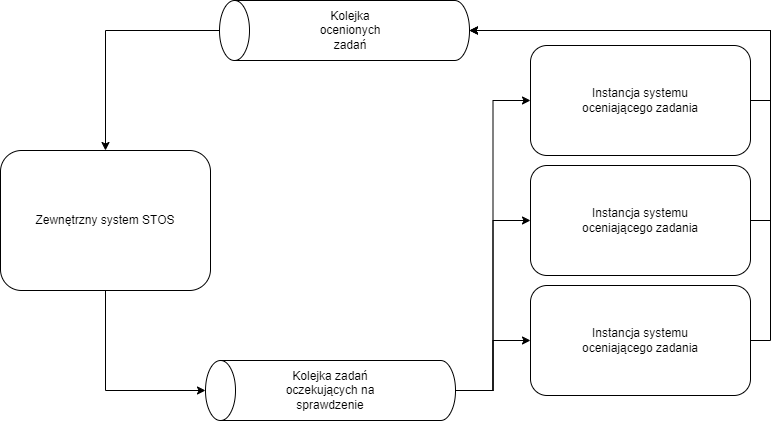
\includegraphics{img/5/system-kolejkowy.png}
		}
		\caption[Schemat komunikacji opartej na systemie kolejkowym. Źródło własne.]{Schemat komunikacji opartej na systemie kolejkowym. Źródło własne.}
    \label{stos-queue}
	\end{center}
\end{figure}